\setchapterpreamble[u]{\margintoc}
\chapter{Evaluations \& Ablation Experiments}
\labch{Ablations}

In this chapter, the results and ablation experiments for to the presented approach shall be showcased.
This is meant to show some weaknesses of each method as well as give a visual understanding of the effects of some losses and parameters.
Together with an interpretation it should help to evaluate the approach in general.

The ablation experiments for the neural renderer will be shorter than those for the optimization procedure.
This is due to the fact that other approaches already introduced neural renderers and showed its capabilities.
Still, some ablation experiments will performed to better evaluate the neural renderer.

It is important to stretch that most evaluations are subjective and readers must judge for themselves if the images appeal to them.

\section{Neural Renderer}
\labsec{ablation_renderer}
\subsection{Results}
First the results of rendering with the neural renderer shall be evaluated a bit more thoroughly than in the previous chapter.

Looking at a series of brushstrokes with different parameters shows that the neural renderer is indeed capable of imitating the functionality of the fluid simulation to a certain degree.
The FID score at the end of the training is $\approx 11 \pm 1$.
\begin{figure*}
    \adjincludegraphics[height=3cm]{series}
    \caption{A series of generated brushstrokes (top) with different parameters with their rendered counter parts (bottom). Each image has only $64\times64\si{\pixel}$ and these images are already upscaled.}
\end{figure*}

Looking further into details, it seems that start and end points are differently rendered which reinforces the perception of an actual brushstroke.
Especially the long tail at the start point, which also fades out is well captured.\\
Other details like the structure of the outline or the structure inside the brushstroke show some discrepancies.
It seems that, even though there is no L2-loss in later training stages, the generated strokes are a bit more blurry.
This could be due to the highly stochastic nature of these details.
Recreating such detailed structures without them getting repetitive, might be a hard task for the generator.
Arguably, the discriminator would easily spot repetitive patterns and penalize them accordingly.\\
Interestingly, this issue is more apparent for renderers which have been trained with L2-loss throughout the whole training.
These brushstrokes show significant signs of blurring, especially in the discussed regions.\\
\begin{figure*}
    \adjincludegraphics[height=3cm]{L2strokes}
    \caption{Generated brushstrokes when the renderer is trained with L2-loss.}
\end{figure*}
The other way around, without any L2-loss in the beginning, the renderer seems to not converge to a good solution.
Especially in early stages of training the generator would then collapse.\\
Presumably, this is case because the behavior of brushstrokes is hard to learn from scratch.
This makes sense, if one thinks about how hard it would be to get a set of 10 variables and find out how they influence the brushstroke without given some hints in the beginning.
Particularly, the stroke path in form of Bézier curve would be hard to learn.

Notably, as training converges, it is hard to assess the quality of brushstrokes and the FID score as evaluation metric comes in handy.

\subsection{Ablation Experiments}
The first ablation experiment that comes to mind, concerns data points outside the training distribution.\\
\reffig{outside} shows a common failure case during optimization, though, other failure cases exist as well.\\
Brushstrokes can also vanish completely or show artifacts.\\

These failure cases are a minor issue as the parameter space is limited to $[0, 1]^10$ yet they occur for certain optimization settings that push parameters ``outside their comfort zone''.\\

\begin{marginfigure}
    \adjincludegraphics[height=3cm]{L2strokes}
    \caption{Failure cases for the generator during optimization.}
    \labfig{outside}
\end{marginfigure}
At last, larger brush sizes have been tested as well.
Both $128\times128 \si{\pixel}$ and $256\times256 \si{\pixel}$ have been trained.
It could be observed that training takes exponentially when having four times the pixels in an image.
\begin{figure*}
    \subfloat[]{%
        \adjincludegraphics[height=4cm]{BS128}
        \labfig{128}%
    }\qquad
    \subfloat[]{%
        \adjincludegraphics[height=4cm]{BS256}
        \labfig{256}%
    }
    \caption{Rendered brushstrokes for (a) $128\times128 \si{\pixel}$ and (b) $256\times256 \si{\pixel}$.}
\end{figure*}

\section{Optimization Procedure}
\labsec{ablation_opt}
\subsection{Results}
It was possible to show that the optimization procedure is capable of approximating images by using a brushstroke representation.

The actual goal was to extract accurate brushstrokes from these images and imitate paintings as well as possible.
Looking as \reffig{ref_examples} shows that, at a first glance, the rendering gives the impression of a painting images, much like the original.\\
\begin{figure*}[!htp]
    \subfloat[The Starry Night]{%
        \adjincludegraphics[height=8cm, trim={0 0 0 {.5\height}},clip]{ablations/reference/starry}
        \labfig{reference:starry}%
    }
    \subfloat[Self-Portrait]{%
        \adjincludegraphics[height=8cm, trim={0 0 0 {.5\height}},clip]{ablations/reference/portrait}
        \labfig{reference:portrait}%
    }
    \caption{Approximated versions of (a) ``The Starry Night'' and (b) a self-portrait by van Gogh.}
    \labfig{ref_examples}
\end{figure*}
However, when looking closer, is quickly becomes apparent that this is not real painting but a generated image.
Looking into a zoomed-in part of the image (\reffig{ref_zoomed}) this becomes even more apparent.
Hence, it was not quite possible to approximate a painting accurately.
\begin{figure*}[!htp]
    \subfloat[The Starry Night]{%
        \adjincludegraphics[height=5cm, trim={100 {.5\height+100} 100 0},clip]{ablations/reference/starry}
        \labfig{zoom:starry}%
    }
    \subfloat[The Starry Night]{%
        \adjincludegraphics[height=5cm, trim={100 100 100 {.5\height}},clip]{ablations/reference/starry}
        \labfig{zoom:starry2}%
    }
    \caption{Zoomed in details of ``The Starry Night'' with it real counterpart).}
    \labfig{ref_zoomed}
\end{figure*}

Considering the same approximations and comparing single brushstrokes, a similar result can be found.\\
Some very recognizable brushstrokes seem to be roughly depicted by a single brushstroke in the approximation.
Nonetheless this is rather rarely the case, and most predicted brushstrokes to not match an actual real-world brushstroke.
Still, it seems as if the general ``flow'' of a region is present in the approximation.
This gives an initial good impression for the approximation which is only debunked after a closer look.\\
When comparing the results to \citeauthor*{LpaintB}'s results, this approach seems to render superior results.
\begin{figure*}[!htp]
    \subfloat{%
        \adjincludegraphics[height=4cm]{starry_lpaintb}
        \labfig{starry:lpaintb}%
    }
    \subfloat{%
        \adjincludegraphics[height=4cm]{starry_paintbot}
        \labfig{starry:paintbot}%
    }
    \subfloat{%
        \adjincludegraphics[height=4cm, trim={0 0 0 {.5\height}},clip]{ablations/reference/starry}
        \labfig{starry:reference}%
    }
    \caption{Comparison of ``The Starry Night`` approximated with by (a) \citeauthor*{LpaintB}~\cite{LpaintB} (a) \citeauthor*{paintbot}~\cite{paintbot}, and (c) this approach.}
    \labfig{approach_comp}
\end{figure*}


Now the brush strokes extraction capabilities will be compared to \citeauthor*{rhythmic}'s and \citeauthor*{lamberti}'s approaches.
The image ``The Little Arlesienne'' has been approximated to compare the results to the patch of the same painting that both authors have provided in their work.
\begin{figure*}[!htp]
    \subfloat{%
        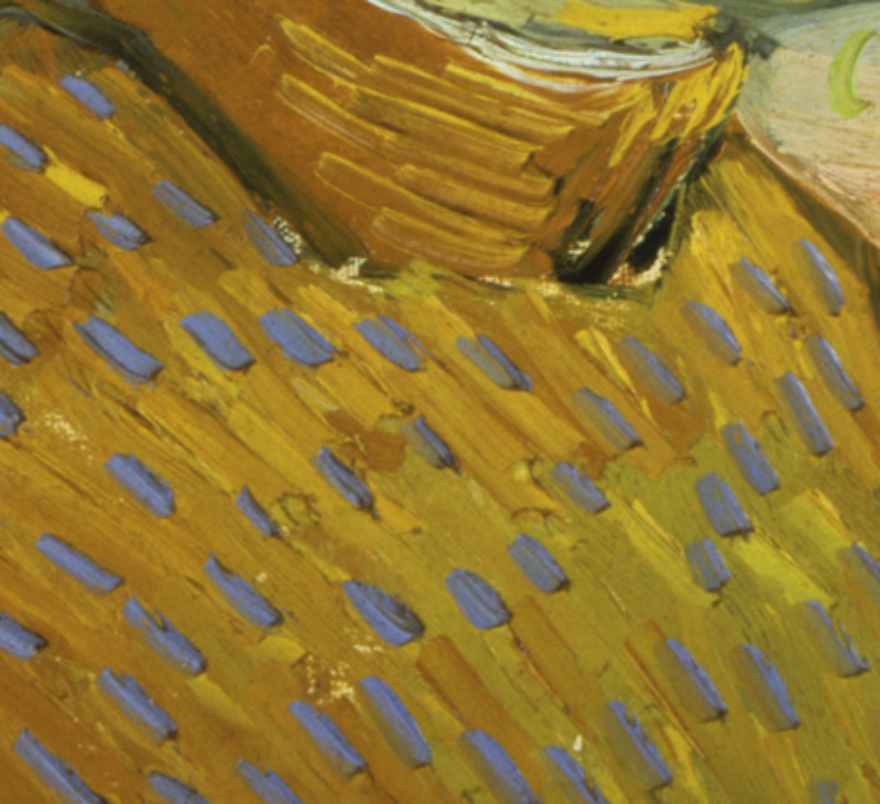
\includegraphics[width=.30\textwidth]{images/cutout_orig}%
        \labfig{_cutout_orig2}%
    }
    \subfloat{%
        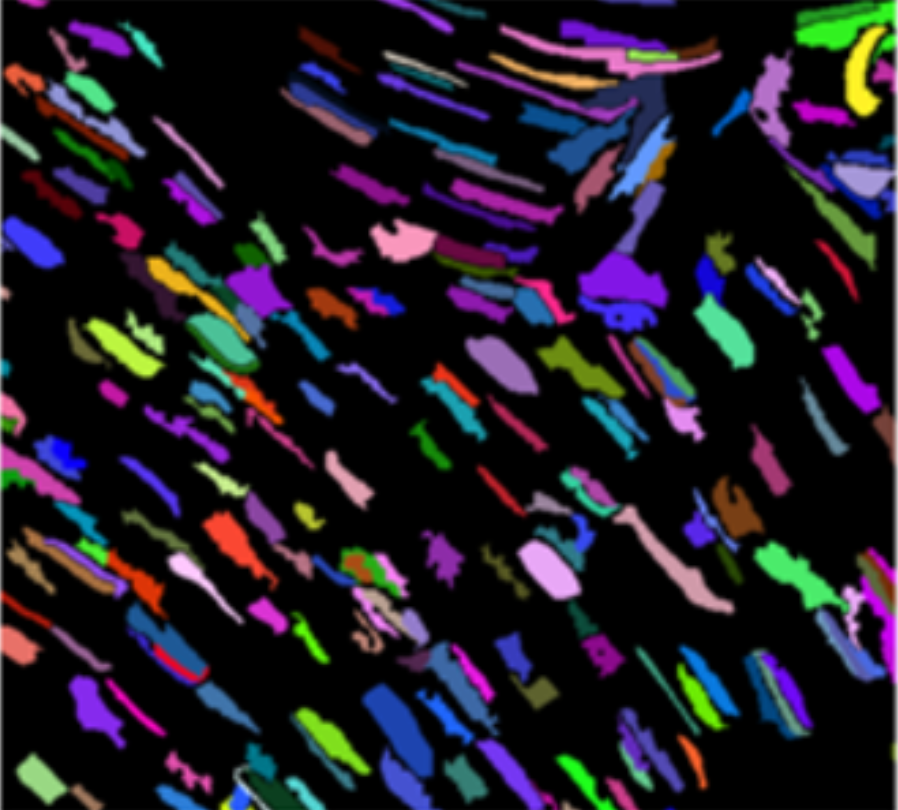
\includegraphics[width=.30\textwidth]{images/cutout_li}%
        \labfig{_cutout_li}%
    }
    \subfloat{%
        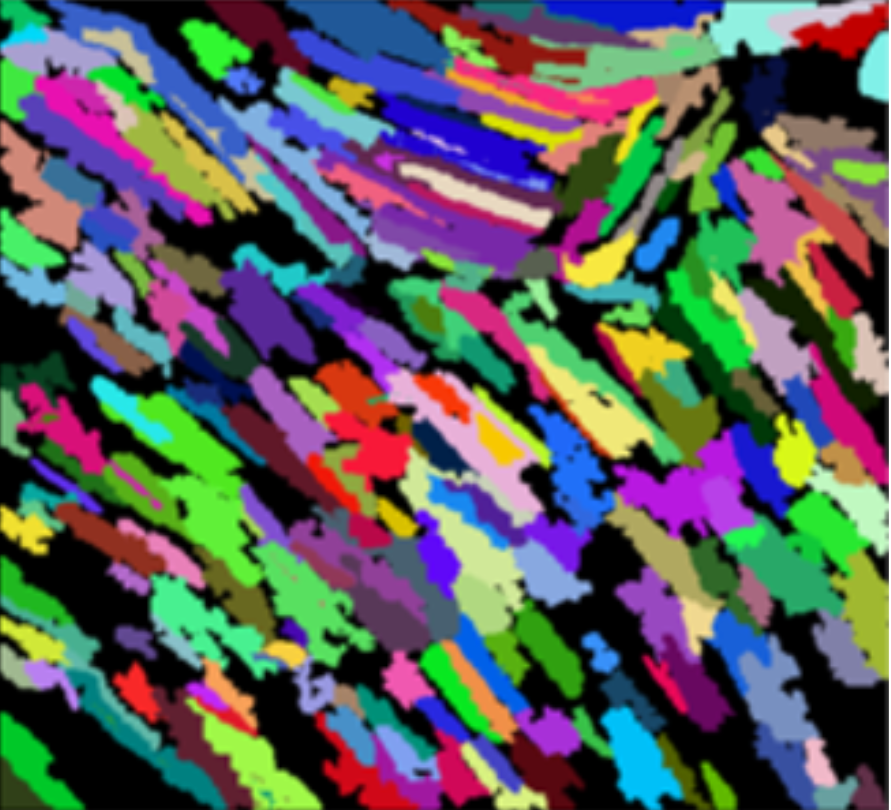
\includegraphics[width=.30\textwidth]{images/cutout_lamberti}%
        \labfig{_cutout_lamberti}%
    }
    \subfloat{%
        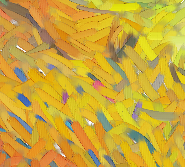
\includegraphics[width=.30\textwidth]{images/cutout_approach}%
        \labfig{_cutout_approach}%
    }
    \subfloat{%
        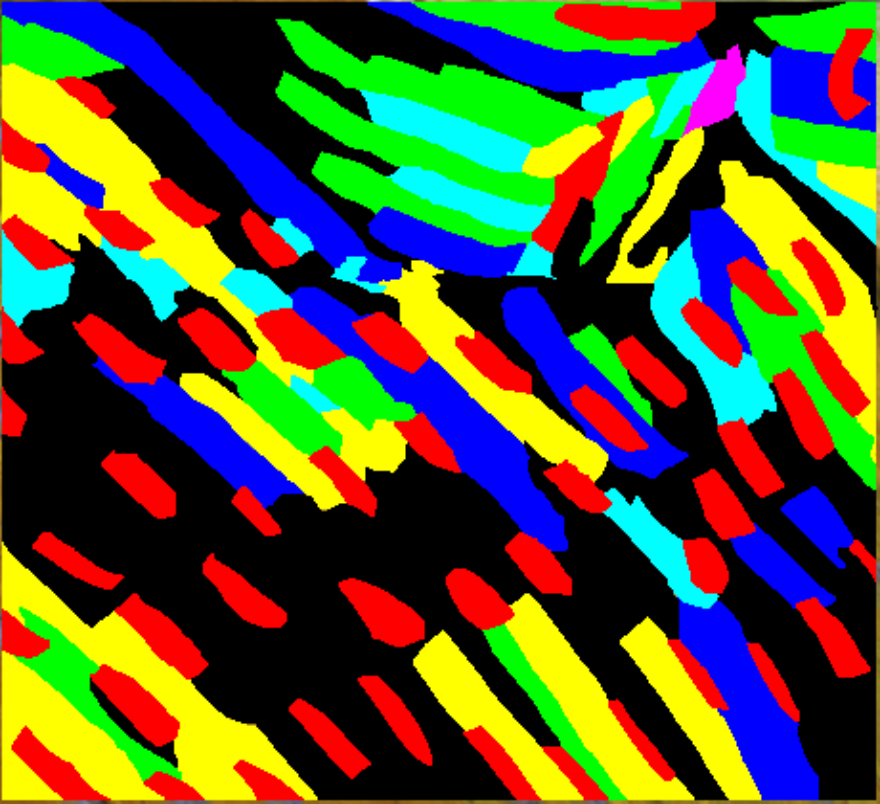
\includegraphics[width=.30\textwidth]{images/cutout_manual}%
        \labfig{_cutout_manual}%
    }
    \caption{Comparison of the same image patch (a) for approaches by (b) \citeauthor*{rhythmic}~\cite{rhythmic}, (c) \citeauthor*{lamberti}~\cite{lamberti}, (d) this thesis and (e) manual labeling~\cite{rhythmic}.}
    \labfig{BSE_comparison}
\end{figure*}
Without labeling the brushstrokes it already becomes apparent that the brushstroke extraction capabilities are worse that those of existing approaches.
It still seems as if the general direction of brushstrokes within this patch is correct.
However, only a handful of brushstrokes have been approximated somewhat correctly.\\
Considering, that the blue brushstrokes build a clear contrast to the yellow background it is even surprising that they have not been better extracted.

At last the painterly rendering capabilities of the approach shall be evaluated.\\
It seems as if this thesis' approach is actually quite capable of generating painterly renderings of photos.
\begin{figure*}[!htp]
    \subfloat{%
        \adjincludegraphics[height=10cm]{images/ablations/reference/tub}%
        \labfig{PR_tub}
    }
    \subfloat{%
        \adjincludegraphics[height=10cm]{images/ablations/reference/GGB}%
        \labfig{PR_GGB}
    }
    \caption{Painterly rendering approximations of this approach for an image of Tübingen (a) and the Golden Gate bridge (b) along with the original photgraphs (c) Source:~\cite{gatys} \& (d)Source:\url{https://commons.wikimedia.org/wiki/File:Golden_Gate_Bridge_.JPG}.}
    \labfig{PR}
\end{figure*}
Notably, the preservation of edges that are important to the content seems to work well, as brushstrokes often align along these edges.
The best example of this are the windows in \reffig{PR_tub}, which are composed of several single straight brushstrokes of different color.
Along with this comes a nice level of abstraction as the tiny details of the windows are lost.\\
The same image also shows a failure case for the painterly rendering with the tree to the left of the image.
Because the tree consists of many thin branches, it is not captured very well.
This is likely caused by the inability of the brushstrokes to become that thin.
Subsequently, only the stem and thick branches are visible.\\
Another problem might be the way the sky is composed.
Here, the brushstrokes seem to not follow any clear pattern which wold be expected if an artist drew the same scene.\\
At last some deviation from the original colors might are visible.
\reffig{PR_GGB} best shows this color inaccuracy at the horizon.

Ultimately, the painterly rendering results are relatively accurate and could be compared to state-of-the-art techniques like those by \citeauthor*{paintbot} or \citeauthor*{hertzmann}

At last, a time-lapse through the optimization process shows very well how the patches are approximated in the early stages of training.
\begin{figure*}[!htp]
    \caption{Time-lapse of the optimization procedure for ``The Starry Night''.}
    \labfig{timelapse}
\end{figure*}

\subsection{Ablation Experiments}
The optimization procedure gives many starting points for ablation experiments.
At first, the effects of each loss will be visually compared.
Then, different initializations will be shown as well as some choices for training
parameters.

%no L2
\begin{figure*}[!htb]
    \subfloat[The Starry Night]{%
        \adjincludegraphics[height=3.5cm, trim={0 0 0 {.5\height}},clip]{ablations/no_l2/starry}
        \labfig{no_l2:starry}%
    }
    \subfloat[Self-Portrait]{%
        \adjincludegraphics[height=3.5cm, trim={0 0 0 {.5\height}},clip]{ablations/no_l2/portrait}
        \labfig{no_l2:portrait}%
    }
    \subfloat[Tübingen]{%
        \adjincludegraphics[height=3.5cm, trim={0 0 0 {.5\height}},clip]{ablations/no_l2/tub}
        \labfig{no_l2:tub}%
    }
    \subfloat[Golden Gate Bridge]{%
        \adjincludegraphics[height=3.5cm, trim={0 0 0 {.5\height}},clip]{ablations/no_l2/GGB}
        \labfig{no_l2:GGB}%
    }
    \caption{Collection of reference images approximated without L2-loss}
    \labfig{no_l2}
\end{figure*}
First off, removing L2-loss shows the expected behavior, as the color accuracy gets worse for all images.
Still abstracted versions of the color are present which is likely caused by the LPIPS loss.
Looking at the ablation experiments without LPIPS loss and just content loss, this intuition is confirmed.\\
Besides the distorted colors the images also show some sparseness, as canvas shines through the brushstrokes.
The is likely also a result of the LPIPS loss, which emphasizes edges over uniformly colored areas.

%no Lpips
\begin{figure*}[!htb]
    \subfloat[The Starry Night]{%
        \adjincludegraphics[height=3.5cm, trim={0 0 0 {.5\height}},clip]{ablations/no_LPIPS/starry}
        \labfig{no_LPIPS:starry}%
    }
    \subfloat[Self-Portrait]{%
        \adjincludegraphics[height=3.5cm, trim={0 0 0 {.5\height}},clip]{ablations/no_LPIPS/portrait}
        \labfig{no_LPIPS:portrait}%
    }
    \subfloat[Tübingen]{%
        \adjincludegraphics[height=3.5cm, trim={0 0 0 {.5\height}},clip]{ablations/no_LPIPS/tub}
        \labfig{no_LPIPS:tub}%
    }
    \subfloat[Golden Gate Bridge]{%
        \adjincludegraphics[height=3.5cm, trim={0 0 0 {.5\height}},clip]{ablations/no_LPIPS/GGB}
        \labfig{no_LPIPS:GGB}%
    }
    \caption{Collection of reference images approximated without LPIPS-loss}
    \labfig{no_lpips}
\end{figure*}
Removing LPIPS loss draws a different picture.
These images show a better color accuracy but seem very blurry as it is often the case when optimizing with L2-loss alone.
Such behavior is expected.

%no KL
\begin{figure*}[!htb]
    \subfloat[The Starry Night]{%
        \adjincludegraphics[height=3.5cm, trim={0 0 0 {.5\height}},clip]{ablations/no_KL/starry}
        \labfig{no_KL:starry}%
    }
    \subfloat[Self-Portrait]{%
        \adjincludegraphics[height=3.5cm, trim={0 0 0 {.5\height}},clip]{ablations/no_KL/portrait}
        \labfig{no_KL:portrait}%
    }
    \subfloat[Tübingen]{%
        \adjincludegraphics[height=3.5cm, trim={0 0 0 {.5\height}},clip]{ablations/no_KL/tub}
        \labfig{no_KL:tub}%
    }
    \subfloat[Golden Gate Bridge]{%
        \adjincludegraphics[height=3.5cm, trim={0 0 0 {.5\height}},clip]{ablations/no_KL/GGB}
        \labfig{no_KL:GGB}%
    }
    \caption{Collection of reference images approximated without explicit brushstroke constraints.}
    \labfig{no_KL}
\end{figure*}
If brushstroke constraints are removed from the collection of losses, there is, in fact, next to failure of the renderer observable.
The only apparent difference seems to be, that brushstrokes seem to get shorter and wider compared to the reference images.
This gives the impression of a slightly different style.

%just content + KL
\begin{figure*}[!htb]
    \subfloat[The Starry Night]{%
        \adjincludegraphics[height=3.5cm, trim={0 0 0 {.5\height}},clip]{ablations/content/starry}
        \labfig{content:starry}%
    }
    \subfloat[Self-Portrait]{%
        \adjincludegraphics[height=3.5cm, trim={0 0 0 {.5\height}},clip]{ablations/content/portrait}
        \labfig{content:portrait}%
    }
    \subfloat[Tübingen]{%
        \adjincludegraphics[height=3.5cm, trim={0 0 0 {.5\height}},clip]{ablations/content/tub}
        \labfig{content:tub}%
    }
    \subfloat[Golden Gate Bridge]{%
        \adjincludegraphics[height=3.5cm, trim={0 0 0 {.5\height}},clip]{ablations/content/GGB}
        \labfig{content:GGB}%
    }
    \caption{Collection of reference images approximated only with perceptual loss and brushstroke constraints.}
    \labfig{content}
\end{figure*}
Minimizing only the perceptual distance to the target image as in \reffig{content} returns a relatively colorless image.
Only edges are depicted accurately which is expected in this case.
This behavior raises the question how style transfer would look if a style loss could be implemented.

%scale of brushstroke to content
\begin{figure*}[!htb]
    \subfloat[The Starry Night]{%
        \begin{tabular}[b]{c}
        \adjincludegraphics[height=3.2cm, trim={0 0 0 {.5\height}},clip]{ablations/upscaled/starry}\\
        \adjincludegraphics[height=3.2cm, trim={0 0 0 {.5\height}},clip]{ablations/downscaled/starry}
        \end{tabular}
        \labfig{downscaled:starry}%
    }
    \subfloat[Self-Portrait]{%
        \begin{tabular}[b]{c}
        \adjincludegraphics[height=3.2cm, trim={0 0 0 {.5\height}},clip]{ablations/upscaled/portrait}\\
        \adjincludegraphics[height=3.2cm, trim={0 0 0 {.5\height}},clip]{ablations/downscaled/portrait}
        \end{tabular}
        \labfig{downscaled:portrait}%
    }
    \subfloat[Tübingen]{%
        \begin{tabular}[b]{c}
        \adjincludegraphics[height=3.2cm, trim={0 0 0 {.5\height}},clip]{ablations/upscaled/tub}\\
        \adjincludegraphics[height=3.2cm, trim={0 0 0 {.5\height}},clip]{ablations/downscaled/tub}
        \end{tabular}
        \labfig{downscaled:tub}%
    }
    \subfloat[Golden Gate Bridge]{%
        \begin{tabular}[b]{c}
        \adjincludegraphics[height=3.2cm, trim={0 0 0 {.5\height}},clip]{ablations/upscaled/GGB}\\
        \adjincludegraphics[height=3.2cm, trim={0 0 0 {.5\height}},clip]{ablations/downscaled/GGB}
        \end{tabular}
        \labfig{downscaled:GGB}%
    }
    \caption{Two collection of reference images with a different image scale. 2x larger scale (top) and 2x smaller scale (bottom) when compared to the original scaling.}
    \labfig{scale}
\end{figure*}
Changing the image scale is particularly interesting in case of painting images.
The resulting approximations show that a different image scale worsens the impression of an actual painting image.\\
Interestingly, the directions of brushstrokes are still similar for the downscaled image which is likely caused by the high contrast between adjacent brushstrokes that van Gogh uses.\\
The upscaled image showcases how many small brushstrokes approximate a single real brushstroke not particularly well.
However, smaller brush strokes like those that make up the ``star-circles'' are better depicted.

%brushstroke density
\begin{figure*}[!htb]
    \subfloat[The Starry Night]{%
        \begin{tabular}[b]{c}
        \adjincludegraphics[height=3.2cm, trim={0 0 0 {.5\height}},clip]{ablations/high_dense/starry}\\
        \adjincludegraphics[height=3.2cm, trim={0 0 0 {.5\height}},clip]{ablations/low_dense/starry}
        \end{tabular}
        \labfig{dense:starry}%
    }
    \subfloat[Self-Portrait]{%
        \begin{tabular}[b]{c}
        \adjincludegraphics[height=3.2cm, trim={0 0 0 {.5\height}},clip]{ablations/high_dense/portrait}\\
        \adjincludegraphics[height=3.2cm, trim={0 0 0 {.5\height}},clip]{ablations/low_dense/portrait}
        \end{tabular}
        \labfig{dense:portrait}%
    }
    \subfloat[Tübingen]{%
        \begin{tabular}[b]{c}
        \adjincludegraphics[height=3.2cm, trim={0 0 0 {.5\height}},clip]{ablations/high_dense/tub}\\
        \adjincludegraphics[height=3.2cm, trim={0 0 0 {.5\height}},clip]{ablations/low_dense/tub}
        \end{tabular}
        \labfig{dense:tub}%
    }
    \subfloat[Golden Gate Bridge]{%
        \begin{tabular}[b]{c}
        \adjincludegraphics[height=3.2cm, trim={0 0 0 {.5\height}},clip]{ablations/high_dense/GGB}\\
        \adjincludegraphics[height=3.2cm, trim={0 0 0 {.5\height}},clip]{ablations/low_dense/GGB}
        \end{tabular}
        \labfig{dense:GGB}%
    }
    \caption{Two collection of reference images with a different brushstroke densities. 2x the reference density (top) and 1/2x the reference density (bottom).}
    \labfig{density}
\end{figure*}
Changing the brushstroke density seem to have a similar effect to scaling the image.
At a higher density many smaller brushstrokes can be seen, at a lower density the brushstrokes become elongated and all feature the maximal width.
Nonetheless, some differences are visible due to the range of the brush size and the parameter constraints.

%high learning rate
\begin{figure*}[!htb]
    \subfloat[The Starry Night]{%
        \adjincludegraphics[height=3.5cm, trim={0 0 0 {.5\height}},clip]{ablations/lr/starry}
        \labfig{lr:starry}%
    }
    \subfloat[Self-Portrait]{%
        \adjincludegraphics[height=3.5cm, trim={0 0 0 {.5\height}},clip]{ablations/lr/portrait}
        \labfig{lr:portrait}%
    }
    \subfloat[Tübingen]{%
        \adjincludegraphics[height=3.5cm, trim={0 0 0 {.5\height}},clip]{ablations/lr/tub}
        \labfig{lr:tub}%
    }
    \subfloat[Golden Gate Bridge]{%
        \adjincludegraphics[height=3.5cm, trim={0 0 0 {.5\height}},clip]{ablations/lr/GGB}
        \labfig{lr:GGB}%
    }
    \caption{Collection of reference images approximated with 10x the original learning rate.}
    \labfig{10xlr}
\end{figure*}
Increasing the learning rate returns the expected sub-optimal solution as the optimizer overshoots good solutions. 

%accuracy
\begin{figure*}[!htb]
    \subfloat[The Starry Night]{%
        \adjincludegraphics[height=3.5cm, trim={0 0 0 {.5\height}},clip]{ablations/no_acc/starry}
        \labfig{no_acc:starry}%
    }
    \subfloat[Self-Portrait]{%
        \adjincludegraphics[height=3.5cm, trim={0 0 0 {.5\height}},clip]{ablations/no_acc/portrait}
        \labfig{no_acc:portrait}%
    }
    \subfloat[Tübingen]{%
        \adjincludegraphics[height=3.5cm, trim={0 0 0 {.5\height}},clip]{ablations/no_acc/tub}
        \labfig{no_acc:tub}%
    }
    \subfloat[Golden Gate Bridge]{%
        \adjincludegraphics[height=3.5cm, trim={0 0 0 {.5\height}},clip]{ablations/no_acc/GGB}
        \labfig{no_acc:GGB}%
    }
    \caption{Collection of reference images approximated with a random ordering.}
    \labfig{acc}
\end{figure*}
Removing accuracy based ordering seems not to make much of a difference.
The reason behind this is probably the fixed ordering that is implemented instead, which is apparently sufficient.

%grid init
\begin{figure*}[!htb]
    \subfloat[The Starry Night]{%
        \adjincludegraphics[height=3.5cm, trim={0 0 0 {.5\height}},clip]{ablations/grid/starry}
        \labfig{grid:starry}%
    }
    \subfloat[Self-Portrait]{%
        \adjincludegraphics[height=3.5cm, trim={0 0 0 {.5\height}},clip]{ablations/grid/portrait}
        \labfig{grid:portrait}%
    }
    \subfloat[Tübingen]{%
        \adjincludegraphics[height=3.5cm, trim={0 0 0 {.5\height}},clip]{ablations/grid/tub}
        \labfig{grid:tub}%
    }
    \subfloat[Golden Gate Bridge]{%
        \adjincludegraphics[height=3.5cm, trim={0 0 0 {.5\height}},clip]{ablations/grid/GGB}
        \labfig{grid:GGB}%
    }
    \caption{Collection of reference images approximated with grid initialization.}
    \labfig{grid_init}
\end{figure*}
Using a grid based initialization also seems to have no visible effect.
This is likely due to the high brushstroke density and the other shortcoming, that outweigh any effect that this layout has.

%too small patch window
\begin{marginfigure}
    \adjincludegraphics[trim={0 0 0 {.5\height}},clip]{smallwindow}
    \caption{Early stage of training with a too-small patch window size}
    \labfig{window_size}
\end{marginfigure}
Having a patch window size which is too small affects the optimization procedure in the early stages the most.
Brushstrokes are driven towards the pixels which lie inside the render window of some part of the render window is cut out.
The result are recognizable lines where the patch window's edges have been.
These line are relatively persistent until they are slowly removed over time when theses strokes are updated again. 

% other artists
\begin{figure*}[!htb]
    \subfloat[]{%
        \adjincludegraphics[height=8cm, trim={0 0 0 {.5\height}},clip]{monalisa}
        \labfig{monalisa}%
    }
    \subfloat[]{%
        \adjincludegraphics[height=8cm, trim={0 0 0 {.5\height}},clip]{bridge}
        \labfig{bridge}%
    }
    \caption{Brushstroke approximation for paintings by other artists. (a) ``The Mona Lisa'' by Leonardo DaVinci (b) ``Bridge over a Pond of Water Lillies`` by Claude Monet}
    \labfig{artists}
\end{figure*}
When considering the approach on works by other artists, a few problem become apparent.\\
First, for fines brushstrokes, as they are present in both paintings, no brushstrokes can be extracted.\\
In case of the Mona Lisa (\reffig{monalisa}) this is even more obvious as brushstrokes are barely visible in the original image.
Nonetheless, the same problems also apply to Monet's painting (\reffig{bridge}).
In the end, both paintings showcase the same problem that previous ablations and the evaluation how well brushstrokes are extracted have already shown.

Ultimately, the optimization procedure behaves very predictable.
The effects of each loss a visible though some mechanics seem to have little to no effect.\\
It seems a bit unfortunate that the brush extraction capabilities are rather limited, but the painterly rendering performance is more promising than originally anticipated.
Subsequently, it would still be interesting to see whether the method could be further improved.

